
\section{The xtsfsp command}
{\tt xtsfsp} estimates spatial stochastic frontier models in the style of \cite{orea2019new} and \cite{galli2022spatial}.

\subsection{Syntax}

Estimation syntax

\begin{stsyntax}
	xtsfsp\
    \depvar\
    \optindepvars,\
	\optional{uhet(\varlist \optional{,noconstant})		
		vhet(\varlist \optional{,noconstant})
		cost
		noconstant
		wy({\it wyspec})
		wx({\it wxspec})
		wu({\it wuspec})
		wv({\it wvspec})
		normalize({\it norm\_method})
		wxvars(\varlist)
		\underbar{init}ial({\it matname})
		mlmodel({\it model\_options})
		mlsearch({\it search\_options})
		mlplot
		mlmax({\it maximize\_options})
		nolog
		mldisplay({\it display\_options})
		level(\num)
		te(\newvarname)
		genwxvars
		delmissing
		constraints(\it constraints)
	}
\end{stsyntax}



\noindent Version syntax

\begin{stsyntax}
	xtsfsp\
	, version
\end{stsyntax}


\noindent Replay syntax

\begin{stsyntax}
	xtsfsp\
	\optional{, level(\num) }
\end{stsyntax}

\subsection{Options}

\hangpara
{\tt uhet(\varlist [,noconstant])} specifies explanatory variables for scaling  function depending on a linear combination of \varlist.  It is required.

\hangpara
{\tt vhet(\varlist [,noconstant])} specifies explanatory variables for idiosyncratic error variance function depending on a linear combination of \varlist. 

\hangpara
{\tt noconstant} suppresses constant term.

\hangpara
{\tt cost} specifies the frontier as a cost function. By default, the production function is assumed.

\hangpara
{\tt wy({\it wyspec})} specifies the spatial weight matrix for lagged dependent variable. The expression is wy($W_1$ $ [W_2 ... W_T]$ [,{\it mata array}]).  By default, the weight matrices are {\tt Sp} objects created by Stata offical command spmatrix. mata declares weight matrices are mata matrices. If one weight matrix is specified, it assumes a time-constant weight matrix. For time-varying cases, $T$ weight matrices should be specified in time order. Alternatively, using array to declare weight matrices are stored in an array.  If only one matrix is stored in the specified array, the time-constant weight matrix is assumed.  Otherwise, the keys of the array specify time information, and the values store time-specific weight matrices.

\hangpara
{\tt wx({\it wxspec})} specifies the spatial weight matrix for lagged independent variable. The expression is the same as {\tt wy({\it wyspec})}.

\hangpara
{\tt wu({\it wuspec})} specifies the spatial weight matrix for lagged independent variable. The expression is the same as {\tt wy({\it wyspec})}.

\hangpara
{\tt wv({\it wvspec})} specifies the spatial weight matrix for lagged independent variable. The expression is the same as {\tt wy({\it wyspec})}.

\hangpara
{\tt normalize({\it norm\_method})} specifies  one of the four available normalization techniques: row, col, minmax, and spectral.

\hangpara
{\tt wxvars(\varlist)} specifies spatially lagged independent variables.


\hangpara
{\tt \underbar{init}ial({\it matname})} specifies  the initial values of the estimated parameters with matrix {\it matname}.

\hangpara
{\tt mlmodel({\it model\_options})} specifies the  {\tt ml model} options.

\hangpara
{\tt mlsearch({\it search\_options})} specifies the  {\tt ml search} options.

\hangpara
{\tt mlplot} specifies using  {\tt ml plot} to search better initial values of spatial dependence parameters.

\hangpara
{\tt mlmax({\it maximize\_options})} specifies the  {\tt ml maximize} options.

\hangpara
{\tt nolog} suppresses the display of the criterion function iteration log.

\hangpara
{\tt mldisplay({\it display\_options})} specifies the  {\tt ml display} options.

\hangpara
{\tt level(\num)} sets confidence level; default is level(95).

\hangpara
{\tt te({\it newvarname})} specifies a new variable name to store the estimates of technical efficiency.

\hangpara
{\tt genwxvars} generates the spatial Durbin terms. It is activated only when {\tt wxvars(\varlist)} is specified.

\hangpara
{\tt delmissing} allows estimation  when missing values are present by  removing the corresponding units from spatial matrix. 

\hangpara
{\tt constraints(\it constraints)}  specifies linear constraints for the estimated model. 


\subsection{Dependency of xtsfsp}
{\tt xtsfsp} depends on the {\it moremata }package contributed by  \cite{BenJann}. If not already installed, you can install it by typing ssc install moremata.


%\section{Examples with simulated data}\label{sec_example}
\section{Examples}\label{sec_example}
In this section, we use simulated data to  exemplify the use of the \textit{xtsfsp} command.  Referring to  \cite{galli2022spatial}, we first consider the $yxuv$-SAR model specified by the following data-generating process (DGP 1) with $i=1,...,300$ and $t=1,..,20$,

\begin{equation}\label{dgp1}
	y_{it} = 0.3W_{i}y_{.t}+2x_{it}+ 0.5W_{i}x_{.t}  + \tilde{v}_{it}-\tilde{u}_{it}
\end{equation}
where $\tilde{v}_{it}$ and $\tilde{u}_{it}$ are defined as in Eqs.\eqref{eq2} and \eqref{eq3} with $\gamma=0.3$, $\tau=0.3$, $Z_{it}=(z_{it},1)'$,$\delta=(2, ln(0.2))'$, $D_{it}=1$ and $\eta = ln(0.2)$. All the spatial matrices for the four spatial components are the same and time-invariant, created from a binary contiguity spatial weight matrix. We generate the exogenous variables $X_{it}$ and $z_{it}$ from the standard normal distribution, respectively. With the sample generated by DGP 1, we can fit the model in the following syntax.

\begin{stlog}
	. use xtsfsp_ex1.dta
{\smallskip}
. xtset id t 
{\smallskip}
Panel variable: id (strongly balanced)
 Time variable: t, 1 to 20
         Delta: 1 unit
{\smallskip}
. * importing spatial weight matrix from xtsfsp_wmat1.mmat
. mata mata matuse xtsfsp_w1.mmat,replace
(loading w1[300,300])
{\smallskip}
. * fitting the model
. xtsfsp y x, uhet(z) wu(w1,mata) wy(w1,mata) wv(w1,mata) wx(w1,mata) wxvars(x) te(te) nolog
{\smallskip}
Spatial frontier model(yxuv-SAR)                     Number of obs =     6,000
                                                     Wald chi2(2)  = 113733.00
Log likelihood = -3953.6034                          Prob > chi2   =    0.0000
{\smallskip}
\HLI{13}{\TOPT}\HLI{64}
           y {\VBAR} Coefficient  Std. err.      z    P>|z|     [95\% conf. interval]
\HLI{13}{\PLUS}\HLI{64}
frontier     {\VBAR}
           x {\VBAR}   2.006736   .0082953   241.91   0.000     1.990477    2.022994
         W_x {\VBAR}   .5457545   .0709898     7.69   0.000     .4066171    .6848919
       _cons {\VBAR}   1.008833   .0460347    21.91   0.000     .9186065    1.099059
\HLI{13}{\PLUS}\HLI{64}
    /lnsigv2 {\VBAR}  -1.566886   .0184019   -85.15   0.000    -1.602953   -1.530819
\HLI{13}{\PLUS}\HLI{64}
uhet         {\VBAR}
           z {\VBAR}   .9858524   .0385881    25.55   0.000      .910221    1.061484
       _cons {\VBAR}  -1.533232   .3361919    -4.56   0.000    -2.192156   -.8743081
\HLI{13}{\PLUS}\HLI{64}
Wy           {\VBAR}
       _cons {\VBAR}     .57773    .062202     9.29   0.000     .4558163    .6996436
\HLI{13}{\PLUS}\HLI{64}
Wv           {\VBAR}
       _cons {\VBAR}   .6066382   .0743834     8.16   0.000     .4608494     .752427
\HLI{13}{\PLUS}\HLI{64}
Wu           {\VBAR}
       _cons {\VBAR}   .6584973   .0938095     7.02   0.000      .474634    .8423606
\HLI{13}{\PLUS}\HLI{64}
         rho {\VBAR}   .2810617   .0286408     9.81   0.000     .2240201    .3361839
       gamma {\VBAR}   .2943177    .033966     8.67   0.000     .2264087    .3593786
         tau {\VBAR}   .3178137    .042162     7.54   0.000     .2329366    .3978845
\HLI{13}{\BOTT}\HLI{64}
Note: Wy:_cons, Wv:_cons and Wu:_cons are the transfromed parameters;
      rho, gamma and tau are their origin metrics in spatial components, repsectively.
      W_(x) represent Spatial Durbin terms W(x)

\end{stlog}

The output shows that the command fits six equations with {\tt ml model}. The frontier equation has three explanatory variables $x_{it}$, $W_ix_{.t}$ and constant. The scaling function uhet() has two explanatory variables $Z_{it}$ and constant.  The equation  /lnsigv2 is constructed for the variance parameter  $\sigma_v^2$ which is transformed by the function $exp(\cdot)$. Three Equations (Wy, Wu, and Wv) handle the spatial dependence parameters $\rho$, $\tau$, and $\gamma$, which are parameterized as Eq.\eqref{para}. We directly include the spatial Durbin term $W_ix_{.t}$ in the frontier equation  (represented as W\_x) such that we do not need to fit a separate equation.  The bottom of the table reports the transformed parameters in the original metric.

Secondly, we consider a restricted model $xuv$-SAR with different spatial weight matrices, one of which is time-varying, and the others are time-constant.  The model is described as DGP 2:
\begin{equation}\label{dgp2}
	y_{it} = 1+2x_{it}+ 0.5W_{i}^{xt}x_{it} + \tilde{v}_{it}+\tilde{u}_{it}, i=1,..,300; t=1,..,10
\end{equation}
where the other parameters are set the same as the DGP 1 except for $W_{i}^{ut}=W_{i}^u$, $W_{i}^{vt}=W_{i}^v$ and $\delta = (4,ln(0.2))'$.  Different from DGP 1, which set the production function frontier, DGP 2 specifies a cost function. The estimation of the model is shown as follows.

\begin{stlog}
	. * importing spatial weight matrices from xtsfsp_w2.mmat
. mata mata matuse xtsfsp_w2.mmat,replace
(loading w1[300,300], w10[300,300], w2[300,300], w3[300,300], w4[300,300], w5[300,300], w6[300,300],
 w7[300,300], w8[300,300], w9[300,300])
{\smallskip}
. local w w1 w2 w3 w4 w5 w6 w7 w8 w9 w10
{\smallskip}
. use xtsfsp_ex2.dta
{\smallskip}
. xtset id t 
{\smallskip}
Panel variable: id (strongly balanced)
 Time variable: t, 1 to 10
         Delta: 1 unit
{\smallskip}
. * initial values for estimated parameters
. mat b=(2,0.5,1,-1.5,4,-1.5,0.6,0.6)
{\smallskip}
. * fitting the model
. xtsfsp y x, cost uhet(z) wu(w2,mata) wv(w1,mata) wxvars(x) wx(`w',mata) init(b) genwxvars nolog
{\smallskip}
Spatial frontier model(xuv-SAR)                       Number of obs =    3,000
                                                      Wald chi2(2)  = 57442.57
Log likelihood = -1911.966                            Prob > chi2   =   0.0000
{\smallskip}
\HLI{13}{\TOPT}\HLI{64}
           y {\VBAR} Coefficient  Std. err.      z    P>|z|     [95\% conf. interval]
\HLI{13}{\PLUS}\HLI{64}
frontier     {\VBAR}
           x {\VBAR}   1.995755   .0083855   238.00   0.000      1.97932     2.01219
         W_x {\VBAR}   .5069275   .0221351    22.90   0.000     .4635435    .5503115
       _cons {\VBAR}   .9917396   .0127293    77.91   0.000     .9667906    1.016689
\HLI{13}{\PLUS}\HLI{64}
    /lnsigv2 {\VBAR}  -1.614693   .0260257   -62.04   0.000    -1.665702   -1.563683
\HLI{13}{\PLUS}\HLI{64}
uhet         {\VBAR}
           z {\VBAR}   3.999532    .002155  1855.94   0.000     3.995308    4.003755
       _cons {\VBAR}   -1.69907   .4472607    -3.80   0.000    -2.575685   -.8224549
\HLI{13}{\PLUS}\HLI{64}
Wv           {\VBAR}
       _cons {\VBAR}   .5877877   .0584046    10.06   0.000     .4733168    .7022585
\HLI{13}{\PLUS}\HLI{64}
Wu           {\VBAR}
       _cons {\VBAR}   .6214134   .0008532   728.34   0.000     .6197412    .6230857
\HLI{13}{\PLUS}\HLI{64}
         tau {\VBAR}   .3010498   .0003879   776.13   0.000     .3002894    .3018098
       gamma {\VBAR}   .2856862   .0268157    10.65   0.000     .2323138    .3373429
\HLI{13}{\BOTT}\HLI{64}
Note: Wv:_cons and Wu:_cons are the transformed parameters;
      gamma and tau are their origin metrics in spatial components, repsectively.
      W_(x) represent Spatial Durbin terms W(x)

\end{stlog}

In the second example, we use {\tt cost} option to specify the type of frontier.  The matrix {\tt b} is used as the initial value for the maximum likelihood estimation. The likelihood function of spatial stochastic frontier models is complicated, and generally difficult to obtain the optimal global solutions. Thus, good initial values would be helpful for fitting spatial stochastic models. Practitioners might fit the non-spatial stochastic models using  {\tt fronteir} and {\tt sfpanel} commands to obtain the initial values of the parameters involved in the frontier and the scaling function and then use the {\tt mlplot} option to search initial values for spatially-correlated parameters.
 
 To show the usage of the \textit{delmissin}g option, we replace the two observation of $Y_{it}$ with missing values and re-run the above codes which gives rise to error information "\textit{missing values found. use delmissing to remove the units from the spmatrix}".  The inclusion of the \textit{delmissing} option addresses this issue and the generated variable \_\_e\_sample\_\_ records the regression sample. 
 
 \begin{stlog}
 	. * replace some observations of y to be missing
. replace y=. if _n==1 | _n==100
(2 real changes made, 2 to missing)
{\smallskip}
. local w w1 w2 w3 w4 w5 w6 w7 w8 w9 w10
{\smallskip}
. * estimation is aborted
. cap noi xtsfsp y x, cost uhet(z) wu(w2,mata) wv(w1,mata) ///
>                     wxvars(x) wx(`w',mata) init(b) nolog
missing values found. use delmissing to remove the units from the spmatrix
invalid syntax
{\smallskip}

 \end{stlog}
  \begin{stlog}
 	. * re-estimation with delmissing option 
. local w w1 w2 w3 w4 w5 w6 w7 w8 w9 w10
{\smallskip}
. cap noi xtsfsp y x, cost uhet(z) wu(w2,mata) wv(w1,mata) wxvars(x) wx(`w',mata) init(b) delmissing nolog
missing values found. The corresponding units are deleted from the spmatrix
{\smallskip}
Spatial frontier model(xuv-SAR)                       Number of obs =    2,998
                                                      Wald chi2(2)  = 57433.89
Log likelihood = -1909.3843                           Prob > chi2   =   0.0000
{\smallskip}
\HLI{13}{\TOPT}\HLI{64}
           y {\VBAR} Coefficient  Std. err.      z    P>|z|     [95\% conf. interval]
\HLI{13}{\PLUS}\HLI{64}
frontier     {\VBAR}
           x {\VBAR}   1.996019    .008386   238.02   0.000     1.979583    2.012455
         W_x {\VBAR}   .5065641   .0221295    22.89   0.000     .4631912    .5499371
       _cons {\VBAR}   .9914628    .012715    77.98   0.000     .9665418    1.016384
\HLI{13}{\PLUS}\HLI{64}
    /lnsigv2 {\VBAR}  -1.615516   .0260341   -62.05   0.000    -1.666542    -1.56449
\HLI{13}{\PLUS}\HLI{64}
uhet         {\VBAR}
           z {\VBAR}   3.999476   .0021537  1857.01   0.000     3.995254    4.003697
       _cons {\VBAR}  -1.698894   .4472168    -3.80   0.000    -2.575423   -.8223653
\HLI{13}{\PLUS}\HLI{64}
Wv           {\VBAR}
       _cons {\VBAR}   .5864895   .0584501    10.03   0.000     .4719295    .7010496
\HLI{13}{\PLUS}\HLI{64}
Wu           {\VBAR}
       _cons {\VBAR}   .6214135   .0008525   728.95   0.000     .6197427    .6230843
\HLI{13}{\PLUS}\HLI{64}
         tau {\VBAR}   .3010498   .0003876   776.78   0.000       .30029    .3018092
       gamma {\VBAR}     .28509   .0268466    10.62   0.000     .2316575    .3368072
\HLI{13}{\BOTT}\HLI{64}
Note: Wv:_cons and Wu:_cons are the transformed parameters;
      gamma and tau are their origin metrics in spatial components, repsectively.
      W_(x) represent Spatial Durbin terms W(x)
      Missing values found
      The regression sample recorded by variable __e_sample__

 \end{stlog}
 
 
 Thirdly, we consider the restricted model $uv$-SAR with time-varying spatial weight matrices and conditional heteroscedasticity of random errors. The DGP 3 is described as
 
 
 
 \begin{equation}\label{dgp3}
 	 \begin{aligned}
 		& y_{it} = 1+2x_{it} + \tilde{v}_{it}-\tilde{u}_{it}, i=1,..,300; t=1,..,10  \\
 		& \sigma_{v,it}^2 = exp(1+d_{it})  \\
 		&  h(Z_{it}'\delta) = \sqrt{exp(1+z_{it})}
 	\end{aligned}
 \end{equation}
 where the other parameters are set the same as the DGP 1 except for $W_{i}^{ut}=W_{i}^{vt}=W_{i}^t$. The following syntax estimates the model alongside the results.
 
 \begin{stlog}
 	. * importing spatial weight matrices from xtsfsp_w3.mmat
. mata mata matuse xtsfsp_w3,replace
(loading w1[300,300], w10[300,300], w2[300,300], w3[300,300], w4[300,300], w5[300,300], w6[300,300], w7[300,300], w8[300,300], w9[300,300])
{\smallskip}
. local w w1 w2 w3 w4 w5 w6 w7 w8 w9 w10
{\smallskip}
. use xtsfsp_ex3.dta
{\smallskip}
. xtset id t
{\smallskip}
Panel variable: id (strongly balanced)
 Time variable: t, 1 to 10
         Delta: 1 unit
{\smallskip}
. xtsfsp y x, wu(`w',mata) wv(`w',mata) uhet(z) vhet(d) nolog
{\smallskip}
Spatial frontier model(uv-SAR)                         Number of obs =   3,000
                                                       Wald chi2(1)  = 7472.38
Log likelihood = -5803.0516                            Prob > chi2   =  0.0000
{\smallskip}
\HLI{13}{\TOPT}\HLI{64}
           y {\VBAR} Coefficient  Std. err.      z    P>|z|     [95\% conf. interval]
\HLI{13}{\PLUS}\HLI{64}
frontier     {\VBAR}
           x {\VBAR}   1.988108   .0229991    86.44   0.000     1.943031    2.033185
       _cons {\VBAR}   .8997916   .0737763    12.20   0.000     .7551927    1.044391
\HLI{13}{\PLUS}\HLI{64}
lnsigv2      {\VBAR}
           d {\VBAR}   .9897965   .0259185    38.19   0.000     .9389972    1.040596
       _cons {\VBAR}   .9950927   .0259519    38.34   0.000      .944228    1.045957
\HLI{13}{\PLUS}\HLI{64}
uhet         {\VBAR}
           z {\VBAR}   1.019351   .0458701    22.22   0.000     .9294473    1.109255
       _cons {\VBAR}   1.122574   .4629594     2.42   0.015     .2151904    2.029958
\HLI{13}{\PLUS}\HLI{64}
Wv           {\VBAR}
       _cons {\VBAR}   .6171649   .0431991    14.29   0.000     .5324961    .7018337
\HLI{13}{\PLUS}\HLI{64}
Wu           {\VBAR}
       _cons {\VBAR}   .6471479   .0703691     9.20   0.000      .509227    .7850688
\HLI{13}{\PLUS}\HLI{64}
         tau {\VBAR}    .299117   .0196647    15.21   0.000     .2601042    .3371547
       gamma {\VBAR}   .3127036   .0317402     9.85   0.000     .2492256    .3735057
\HLI{13}{\BOTT}\HLI{64}
Note: Wv:_cons and Wu:_cons are the transformed parameters
      gamma and tau are their origin metrics in spatial components, repsectively.

 \end{stlog}
 
 
Finally, we use the real data to show how to conduct the empirical studies with the models and the command  described above. We collect the raw data on China's provinces from the CSMAR database including  GDP (denoted as Y), investment, labor force (denoted as L), the ratio of government expenditure to GDP (denoted as fiscal), the ratio of FDI to GDP (denoted as fdi),, and the trade as a share of GDP (denoted as trade).  All nominal variables are deflated into the constant price in 1997.  The capital stocks by provinces are estimated  with the PIM method.  The production function is approximated by the translog function and the scaling function of the inefficiency term is assumed to be determined by the ratio of government expenditure to GDP, the ratio of FDI to GDP, and the trade as a share of GDP . 

 \begin{stlog}
	. * Translate shapefile to Stata format
. cap spshape2dta province
{\smallskip}
. 
. use province 
{\smallskip}
. drop if _ID == 26 | _ID>31
(4 observations deleted)
{\smallskip}
. spset 
{\smallskip}
      Sp dataset: province.dta
Linked shapefile: province_shp.dta
            Data: Cross sectional
 Spatial-unit ID: _ID
     Coordinates: _CX, _CY (planar)
{\smallskip}
. * Create spatial contiguity matrix
. spmatrix create contiguity w_con, normalize(none) 
  weighting matrix in w_con contains 1 island
{\smallskip}
. * Obtain spatial matrix as Mata matrix wm from w_con 
. spmatrix matafromsp wm id = w_con
{\smallskip}
. * Match the iland (_ID = 21) with the nearest province(_ID =19)
. mata: wm[19,21]=1
{\smallskip}
. mata: wm[21,19]=1
{\smallskip}
. * Create spmatrix w_con from Mata matrix wm and rwo-normalized the matrix 
. spmatrix spfrommata w_con= wm id, normalize(row) replace
{\smallskip}
. * Obtain the new spatial matrix as Mata matrix wm from w_con 
. spmatrix matafromsp wm id = w_con
{\smallskip}
. 
. use chnempirical.dta,clear
{\smallskip}
. * Generate varables for the translog function
. qui translog Y K L , time(year) norm 
{\smallskip}
. global x  lnK lnL _t lnK_lnL _t_lnK _t_lnL _t_2 lnK_2 lnL_2
{\smallskip}
. global z fiscal trade fdi
{\smallskip}
. * Fit the model with frontier command
. frontier lnY \$x,uhet(\$z) nolog
{\smallskip}
Stoc. frontier normal/half-normal model               Number of obs =      630
                                                      Wald chi2(9)  = 33273.49
Log likelihood = 307.21728                            Prob > chi2   =   0.0000
{\smallskip}
\HLI{13}{\TOPT}\HLI{64}
         lnY {\VBAR} Coefficient  Std. err.      z    P>|z|     [95\% conf. interval]
\HLI{13}{\PLUS}\HLI{64}
lnY          {\VBAR}
         lnK {\VBAR}   .7939407    .020148    39.41   0.000     .7544513      .83343
         lnL {\VBAR}   .2423919   .0152754    15.87   0.000     .2124527    .2723312
          _t {\VBAR}  -.0159651   .0029995    -5.32   0.000     -.021844   -.0100862
     lnK_lnL {\VBAR}  -.0239117   .0463983    -0.52   0.606    -.1148507    .0670274
      _t_lnK {\VBAR}   .0385162   .0100006     3.85   0.000     .0189153     .058117
      _t_lnL {\VBAR}  -.0212483   .0070556    -3.01   0.003     -.035077   -.0074197
        _t_2 {\VBAR}  -.0064186   .0009174    -7.00   0.000    -.0082166   -.0046206
       lnK_2 {\VBAR}  -.0151869   .0327529    -0.46   0.643    -.0793815    .0490077
       lnL_2 {\VBAR}  -.0604274    .031823    -1.90   0.058    -.1227993    .0019444
       _cons {\VBAR}   .3105853   .0138557    22.42   0.000     .2834287    .3377419
\HLI{13}{\PLUS}\HLI{64}
lnsig2v      {\VBAR}
       _cons {\VBAR}  -4.491706   .0912372   -49.23   0.000    -4.670528   -4.312885
\HLI{13}{\PLUS}\HLI{64}
lnsig2u      {\VBAR}
      fiscal {\VBAR}   .0724787   .0116298     6.23   0.000     .0496848    .0952726
       trade {\VBAR}  -.0790757   .0165127    -4.79   0.000      -.11144   -.0467115
         fdi {\VBAR}  -.0262741    .006819    -3.85   0.000    -.0396391   -.0129091
       _cons {\VBAR}  -2.964112   .3476526    -8.53   0.000    -3.645499   -2.282726
\HLI{13}{\PLUS}\HLI{64}
     sigma_v {\VBAR}   .1058372   .0048281                      .0967849    .1157361
\HLI{13}{\BOTT}\HLI{64}
{\smallskip}
. * Predict the inefficiency term and efficiency scores
. predict double uhat, u
{\smallskip}
. gen double te0 = exp(-u) 
{\smallskip}
. * Store the estimated parameters
. mat b0=e(b)
{\smallskip}
. 
. * Fit the model with xtsfsp command
. xtset _ID year
{\smallskip}
Panel variable: _ID (strongly balanced)
 Time variable: year, 1997 to 2017
         Delta: 1 unit
{\smallskip}
. mat b1 = b0,0.6,0.6,0.6
{\smallskip}
. xtsfsp lnY \$x, uhet(\$z) wy(wm,mata) wu(wm,mata) wv(wm,mata) init(b1) te(tesp1) nolog 
{\smallskip}
Spatial frontier model(yuv-SAR)                       Number of obs =      630
                                                      Wald chi2(9)  = 16704.73
Log likelihood = 328.51183                            Prob > chi2   =   0.0000
{\smallskip}
\HLI{13}{\TOPT}\HLI{64}
         lnY {\VBAR} Coefficient  Std. err.      z    P>|z|     [95\% conf. interval]
\HLI{13}{\PLUS}\HLI{64}
frontier     {\VBAR}
         lnK {\VBAR}   .6720836   .0259441    25.91   0.000     .6212341    .7229331
         lnL {\VBAR}   .3390601   .0185192    18.31   0.000      .302763    .3753571
          _t {\VBAR}   .0141493   .0051647     2.74   0.006     .0040267    .0242719
     lnK_lnL {\VBAR}   .0075504    .051805     0.15   0.884    -.0939855    .1090864
      _t_lnK {\VBAR}   .0425662   .0115137     3.70   0.000     .0199998    .0651326
      _t_lnL {\VBAR}  -.0034571   .0079979    -0.43   0.666    -.0191327    .0122186
        _t_2 {\VBAR}  -.0069112   .0013048    -5.30   0.000    -.0094686   -.0043539
       lnK_2 {\VBAR}  -.0875718   .0344022    -2.55   0.011     -.154999   -.0201446
       lnL_2 {\VBAR}  -.0388746   .0377404    -1.03   0.303    -.1128443    .0350952
       _cons {\VBAR}   .4968023    .043107    11.52   0.000     .4123142    .5812903
\HLI{13}{\PLUS}\HLI{64}
    /lnsigv2 {\VBAR}  -4.025468   .0581939   -69.17   0.000    -4.139526    -3.91141
\HLI{13}{\PLUS}\HLI{64}
uhet         {\VBAR}
      fiscal {\VBAR}   .0098788   .0056888     1.74   0.082     -.001271    .0210287
       trade {\VBAR}  -.0911438   .0213384    -4.27   0.000    -.1329663   -.0493212
         fdi {\VBAR}  -.0185831   .0100212    -1.85   0.064    -.0382243    .0010582
       _cons {\VBAR}  -1.963808   .3894655    -5.04   0.000    -2.727146   -1.200469
\HLI{13}{\PLUS}\HLI{64}
Wy           {\VBAR}
       _cons {\VBAR}  -.0467557   .0362548    -1.29   0.197    -.1178138    .0243023
\HLI{13}{\PLUS}\HLI{64}
Wv           {\VBAR}
       _cons {\VBAR}  -.0671769   .1600686    -0.42   0.675    -.3809057    .2465518
\HLI{13}{\PLUS}\HLI{64}
Wu           {\VBAR}
       _cons {\VBAR}   1.280422   .2367245     5.41   0.000       .81645    1.744393
\HLI{13}{\PLUS}\HLI{64}
         rho {\VBAR}  -.0233713   .0181157    -1.29   0.197     -.058833    .0121493
       gamma {\VBAR}  -.0335725   .0799361    -0.42   0.674    -.1881642     .122643
         tau {\VBAR}   .5649866   .0805643     7.01   0.000     .3869258    .7024182
\HLI{13}{\BOTT}\HLI{64}
Note: Wy:_cons, Wv:_cons and Wu:_cons are the transfromed parameters;
      rho, gamma and tau are their origin metrics in spatial components, repsectively.
{\smallskip}
. scalar loglikehood1 =  e(ll)
{\smallskip}
. mat b1 = b0,0.6
{\smallskip}
. xtsfsp lnY \$x, uhet(\$z)  wu(wm,mata)  init(b1) te(tesp2)  nolog
{\smallskip}
Spatial frontier model:u-SAR                          Number of obs =      630
                                                      Wald chi2(9)  = 16174.91
Log likelihood = 327.60816                            Prob > chi2   =   0.0000
{\smallskip}
\HLI{13}{\TOPT}\HLI{64}
         lnY {\VBAR} Coefficient  Std. err.      z    P>|z|     [95\% conf. interval]
\HLI{13}{\PLUS}\HLI{64}
frontier     {\VBAR}
         lnK {\VBAR}    .672366   .0264662    25.40   0.000     .6204932    .7242388
         lnL {\VBAR}   .3392661   .0184417    18.40   0.000     .3031209    .3754113
          _t {\VBAR}   .0114801    .004803     2.39   0.017     .0020664    .0208937
     lnK_lnL {\VBAR}   .0128618   .0467126     0.28   0.783    -.0786932    .1044169
      _t_lnK {\VBAR}   .0422561   .0108054     3.91   0.000     .0210779    .0634344
      _t_lnL {\VBAR}  -.0027543   .0074782    -0.37   0.713    -.0174113    .0119027
        _t_2 {\VBAR}  -.0066348   .0012629    -5.25   0.000      -.00911   -.0041595
       lnK_2 {\VBAR}  -.0915034   .0326073    -2.81   0.005    -.1554126   -.0275942
       lnL_2 {\VBAR}  -.0395255   .0328292    -1.20   0.229    -.1038696    .0248185
       _cons {\VBAR}   .4644181   .0315665    14.71   0.000     .4025489    .5262874
\HLI{13}{\PLUS}\HLI{64}
    /lnsigv2 {\VBAR}  -4.013496   .0575493   -69.74   0.000     -4.12629   -3.900701
\HLI{13}{\PLUS}\HLI{64}
uhet         {\VBAR}
      fiscal {\VBAR}   .0097757      .0055     1.78   0.076     -.001004    .0205555
       trade {\VBAR}  -.0869182   .0204711    -4.25   0.000    -.1270408   -.0467956
         fdi {\VBAR}  -.0133135   .0090702    -1.47   0.142    -.0310908    .0044638
       _cons {\VBAR}  -1.986602   .3822161    -5.20   0.000    -2.735732   -1.237472
\HLI{13}{\PLUS}\HLI{64}
Wu           {\VBAR}
       _cons {\VBAR}    1.07423   .1922999     5.59   0.000     .6973292    1.451131
\HLI{13}{\PLUS}\HLI{64}
         tau {\VBAR}    .490752   .0729815     6.72   0.000     .3351572    .6202829
\HLI{13}{\BOTT}\HLI{64}
{\smallskip}
. scalar loglikehood2 =  e(ll)
{\smallskip}
. local lrtest = -2*(loglikehood2-loglikehood1)
{\smallskip}
. local pvalue = 1- chi2(2,`lrtest')
{\smallskip}
. display "Likelihood-ratio test: LR chi2(2) = `lrtest', Prob > chi2 = `pvalue'"
Likelihood-ratio test: LR chi2(2) = 1.807357699424301, Prob > chi2 = .4050766989379054
{\smallskip}
. 
. * Plot the density of estimates of technical efficiency from different models
. twoway (kdensity te0, color(black) lpattern(solid)) ///
>        (kdensity tesp1,color(red) lpattern(dash))   ///
>            (kdensity tesp2,color(blue) lpattern(longdash)),  ///
>         legend(pos(10) ring(0) label(1 Non-spatial Stoc. Frontier) ///
>         label(2 Spatial Stoc. Frontier:yuv) label(3 Spatial Stoc. Frontier:u)) ///
>         xtitle("Technical Efficiency") ytitle("Density")
{\smallskip}
. graph2tex, epsfile("../output/fig1") caption(Distribution of efficency scores) label(fig1)
\% exported graph to ../output/fig1.eps
\% We can see in Figure \\ref{\lbr}fig:fig1{\rbr} that
\\begin{\lbr}figure{\rbr}[h]
\\begin{\lbr}centering{\rbr}
  \\includegraphics[height=3in]{\lbr}../output/fig1{\rbr}
  \\caption{\lbr}Distribution of efficency scores{\rbr}
  \\label{\lbr}fig:fig1{\rbr}
\\end{\lbr}centering{\rbr}
\\end{\lbr}figure{\rbr}
{\smallskip}
. 

\end{stlog}

To construct the spatial weight matrix,  we use the geographic data \footnote{They include province.shp and province.dbf.} and use the Stata command shshape2dta for conversion. We drop some units with heavily missing values (drop  if \_ID==26 | \_ID>31 ).  Based on the generated province.dta, we construct the spatial contiguity matrix with Stata Official spmatrix routines \footnote{The community-contributed command spwmatrix by \citep{Wilner2010} is also a powerful tool for creating spatial weight matrix in Stata}. As \_ID 26 is an iland so that we define its contiguity unit with the nearest one. As such, we extract the spatial weight matrix as wm in the Mata environment from the spmatrix object w\_con and assign the elements wm[19,21] and wm[21,19] with one.  Furthermore, we use the spmatrix routine to standardize the matrix.  Now, the spmatrix object w\_con can be used for our command xtsfsp. Alternatively, we can put the new w\_con into the Mata environment as wm.  After the preparation of the spatial weight matrix, we fit the models with the  empirical data. 

We begin with fitting a non-spatial stochastic frontier model with Stata official comamnd frontier. We predict the efficiency scores stored in the new variable te0  and extract the estimates of the parameters to serve as the initial values in spatial stochastic frontier models.  Then we consider three source of spatial dependence. The estimated results show that the spatial correlation coefficients for the lag of dependent variable and the random errors are statistically insignificant at the 10\% level. As such, we consider a restricted model with spatial dependence in the inefficient term.  Since the restricted model is nested in the previous model, we also conduct the likelihood ratio test. The result documents that the null hypothesis the restricted model can not be rejected. The significant of $\tau$  indicates the positive spatial spillovers of technical efficiency. Figure 1 shows the distribution of efficiency scores estimated by different models. 

\begin{figure}[h]
	\begin{centering}
		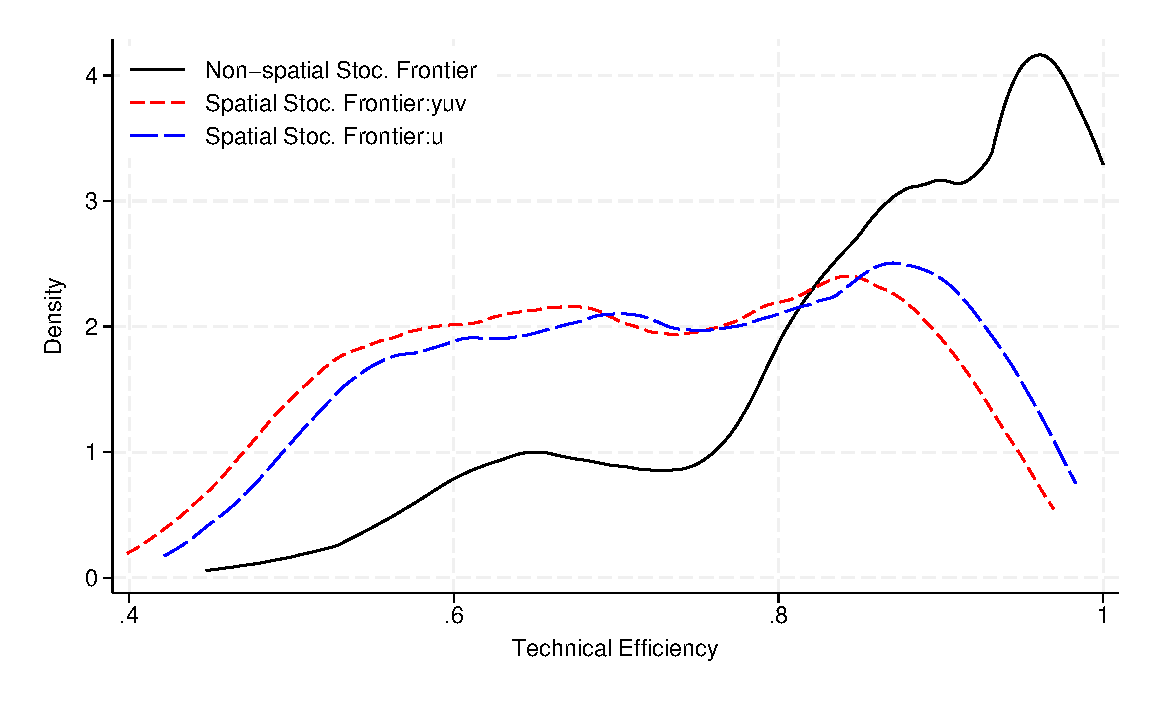
\includegraphics[height=3in]{../output/fig1}
		\caption{Distribution of efficiency scores}
		\label{fig:fig1}
	\end{centering}
\end{figure}




 
 
%\section{Empirical applications}

\section{Conclusion}\label{sec_conclusion}

Geospatial units are not isolated or separated but connected. For example, the economic trade, social activities, and cultural exchange between different regions affect each other. Such spatial interdependence challenges the traditional econometric methods, which generally assume cross-sectional independence. Spatial econometrics is developed to handle spatial correlation.  This article presented a community-contributed command for fitting spatial stochastic frontier models with different sources of spatial dependence \citep{galli2022spatial,orea2019new}. We hope the developed command can provide some convenience to practitioners and reduce the difficulty of model applications, thereby promoting sound empirical research. 

Finally, there are some limitations that should be duly noted.  First, despite the excellent flexibility of the spatial stochastic frontier models and our command introduced above, they fully parameterize the spatial structure, the frontier function and the distribution of random errors and inefficiency term in the spirit of stochastic frontier models and spatial econometrics. The model mispecifications are the potential costs. Some theoretical works devoted into relax the parametric assumptions are particularly valuable. Secondly, the models require prior information on the spatial weight matrices. The different choices of the spatial weight matrices might lead to various results.  Internalizing the spatial weight matrices. in the spatial stochastic frontier models is still an open issue. Thirdly, the numerical computation for the MLE of the spatial stochastic frontier model is very complicated. When the spatial weight matrix is large and the time-varying spatial weight matrix is taken into account, the  estimation is very time consuming because the matrix has to be inverted repeatedly. 




\section{Acknowledgments}
Kerui Du thanks the financial support of the National Natural Science Foundation of China (72074184).  We are grateful to Federica Galli for his Matlab codes, Federico Belotti, Silvio Daidone, Giuseppe Ilardi and Vincenzo Atella for the sfcross/sfpanel package, Mustafa U. Karakaplan for the sfkk package, and Jan Ditzen, William Grieser and Morad Zekhnini for the nwxtregress package which inspired our design of the {\tt xtsfsp} command. 



\endinput
